% DO NOT ALTER OR REMOVE COPYRIGHT NOTICES OR THIS HEADER.
%
% Copyright 1997-2007 Sun Microsystems, Inc. All rights reserved.
%
% The contents of this file are subject to the terms of either the GNU
% General Public License Version 2 only ("GPL") or the Common
% Development and Distribution License("CDDL") (collectively, the
% "License"). You may not use this file except in compliance with the
% License. You can obtain a copy of the License at
% http://www.netbeans.org/cddl-gplv2.html
% or nbbuild/licenses/CDDL-GPL-2-CP. See the License for the
% specific language governing permissions and limitations under the
% License.  When distributing the software, include this License Header
% Notice in each file and include the License file at
% nbbuild/licenses/CDDL-GPL-2-CP.  Sun designates this
% particular file as subject to the "Classpath" exception as provided
% by Sun in the GPL Version 2 section of the License file that
% accompanied this code. If applicable, add the following below the
% License Header, with the fields enclosed by brackets [] replaced by
% your own identifying information:
% "Portions Copyrighted [year] [name of copyright owner]"
%
% Contributor(s):
%
%The Original Software is the LaTeX module.
%The Initial Developer of the Original Software is Jan Lahoda.
%Portions created by Jan Lahoda are Copyright 2002-2004.
%All Rights Reserved.
%
% If you wish your version of this file to be governed by only the CDDL
% or only the GPL Version 2, indicate your decision by adding
% "[Contributor] elects to include this software in this distribution
% under the [CDDL or GPL Version 2] license." If you do not indicate a
% single choice of license, a recipient has the option to distribute
% your version of this file under either the CDDL, the GPL Version 2 or
% to extend the choice of license to its licensees as provided above.
% However, if you add GPL Version 2 code and therefore, elected the GPL
% Version 2 license, then the option applies only if the new code is
% made subject to such option by the copyright holder.
%
%Contributor(s): Jan Lahoda

\documentclass{article}
\usepackage{color}
\usepackage{graphicx}
\usepackage{html}
\usepackage{xspace}

\newcommand{\lenv}{\LaTeX{} authoring environment\xspace}
\newcommand{\done}{\textcolor[rgb]{0.0,1.0,0.0}{DONE}}

\title{\lenv}

\author{Jan Lahoda}

\begin{document}

\maketitle

\section{Introduction}

\label{ch:intro}

The \LaTeX{} authoring environment is an Integrated Development Environment
(IDE) for \LaTeX{}, written in Java\footnote{In fact, the authoring tool is
only an add-on module for an existing Java IDE NetBeans.}. Powerful features
supporting editing \LaTeX{} code are provided.

\subsection{What It Is and What It Is Not}

This editor supports editing of plain \LaTeX{} code. It has quite advanced features.

It is NOT a WYSIWYG (or WYSIWYM --- What You See Is What You Meant) editor.

\subsection{Requirements}

\label{sec:req}

\begin{itemize}
\item{min. 128MB RAM (256MB recommended)}
\item{approx. 80MB free disk space}
\item{JDK1.4.1 or later}
\end{itemize}

\subsection{Features}

\label{sec:features}

\begin{description}
\item[syntax highlighting for \LaTeX{} text]{\LaTeX{} commands, arguments and many more}
\item[integrated spell checker and corrector]{words not in the dictionary are underlined}
\item[interactive code completion]{is provided for a wide range of text elements:
\begin{itemize}
\item{(subset of) LaTeX{} commands and arguments of these}
\item{natural language words}
\item{\verb+\ref+ argument}
\item{\verb+\cite+ argument (parses BiBTeX file)}
\item{\verb+\documentclass+ and \verb+\usepackage+ arguments}
\end{itemize}
}
\item[help on LaTeX{} commands]{provided instantly in the editor}
\item[reverse search]{}
\item[\LaTeX{} model]{and parser with error recovery, providing fast error info}
\item[automata GUI editor]{editor for Vaucanson}
\item[code folding]{}
\item[\LaTeX{} structure]{}
\item[mathematical symbols list]{}
%\item[\LaTeX{} model]{}
\end{description}

\subsection{Installation}

%\chapter{Starting to Work}
%
%In this chapter you should learn how to do basic operations using the \lenv{}.

%\chapter{Usage}

%\label{ch:usage}

\section{Project System}

\label{}

%\section{Syntax highlighting}
%
%\label{sec:high}

\section{Code completion}

\label{sec:completion}

Code completion can be invoked using \verb+Ctrl-Space+ shortcut. The content
of the code completion vary depending on the actual context. In each context
a prefix is defined, and only possibilities beginning with the appropriate
prefix are shown.

Basically, there are following situations when the code completion offers results:
\begin{itemize}
\item{plain text}
\item{command}
\item{command argument}
\end{itemize}

The first two situations offer the list words and the list of commands, respectively.

The last situation is much more complicated. If the command corresponding to
the argument is one of special commands (\verb+\cite+, \verb+\ref+,
\verb+\usepackage+, , \verb+\documentclass+),
special results (as described below) are shown. If there is a list of allowed
values of this arguments, this list is offered. Otherwise, no code completion
is provided.

%TODO: arguments must be closed !!!

\subsection{Citations}

\label{ssec:citations}

The code completion for the \verb+\cite+ command provides all publications in all
requested BiBTeX databases. The BiBTeX database is added to the search, if it is
mentioned in an \verb+\bibliography+ command.

The code completion for \verb+\cite+ currently does not recognise \verb+thebibligoraphy+
environment.

\subsection{References}

\label{ssec:references}

The code completion for the \verb+\ref+ command are all found labels altogether with
the guessed captions.

\subsection{Document Classes and Packages}

\label{ssec:docclasses:packages}

The code completion for the first (non-mandatory) argument of the \verb+\usepackage+
and \verb+\documentclass+ command is the list of all known options for given package
or document class, respectively.

The code completion for the second (mandatory) argument of the \verb+\usepackage+
and \verb+\documentclass+ command is the list of all known packages and document
classes.

It is recommended to fill out the second mandatory argument of these
commands at the beginning and after fill the first non-mandatory argument.

\section{Spell Checker}
\label{sec:spell}

The spell checker is integrated in the \LaTeX editor. Each word in the document
is checked against the dictionary and underline if it is not valid. Interactive
spell-correction is also available.

\subsection{Spell Checker}

\label{ssec:spell:checker}

Spell Checker checks spelling of words against the dictionary. There are three
possible results of the check:

\begin{itemize}
\item{the word is correct. In this case, it is
not underlined.}
\item{the word is a prefix of another word in the dictionary. In this case, it is
underlined by the gray waveline.}
\item{the word is not correct (it does not fall into previous categories).
In this case, it is underlined by the red waveline.}
\end{itemize}

\subsection{Spell Correction}

\label{ssec:spell:correction}

The editor also allows to correct spelling errors interactively. Simply point
the mouse over an incorrectly spelled word, press right mouse button and
select ``Spelling'' in the pop-up menu. A list of words similar to the incorrect
one will appear. When a word is chosen from this list, it immediately replaces the
original incorrect word.

\subsection{Selecting dictionary}

For each document, a dictionary is chosen according to locale of the document.
By default, each document has set \emph{default} locale, which maps to the
system default locale. The locale of a document can be changed using
\emph{LaTeX$\rightarrow$Change Language} menu item. Under this menu, the locales
of all installed dictionaries, the \emph{Default} locale and the \emph{Other} are
shown. If a dictionary is found for a given locale, it is used for spell checking
(see Sections~\ref{ssec:spell:checker} and~\ref{ssec:spell:correction}).
If none dictionary is found, the spell checking is turned off the document.

%TODO: Algorithm for finding of correct dictionary.

\subsection{Adding dictionaries}

%TODO: spell checker vs. spell corrector

\section{Structural View}

\label{sec:structural:view}

The Structural View shows an overview on the structure of the document.
The structure is presented as a tree (see Figure~\ref{fig:structural:view}).
All nodes has the
Go~To~Source action, which jumps to the corresponding point in the source.

\begin{figure}
\caption{Structural View}
\label{fig:structural:view}
\htmlimage{scale=1}
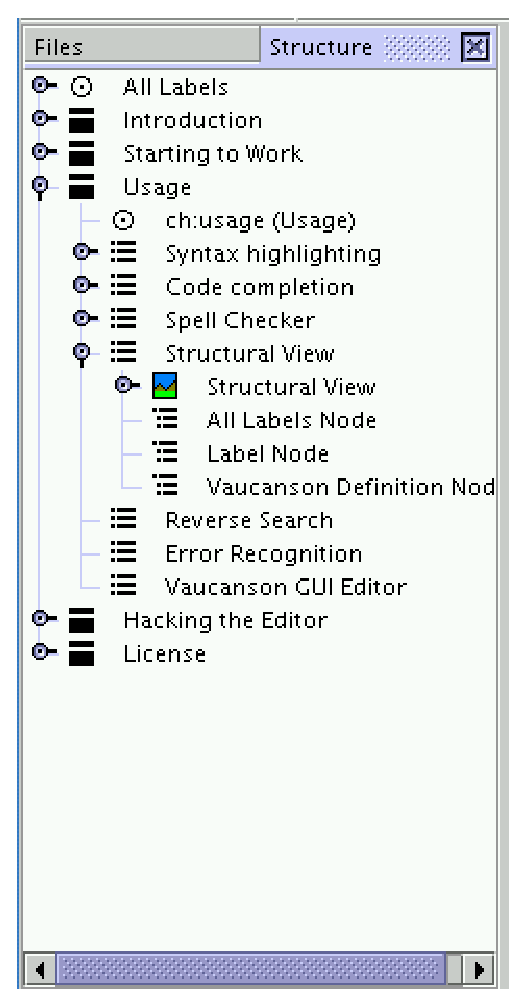
\includegraphics[]{structural_view.eps}
\end{figure}

There are some special types of nodes in the tree, described below.

\subsection{All Labels Node}

\label{ssec:all:labels:node}

Under this node, all labels found in the document are listed.

\subsection{Label Node}

\label{ssec:label:node}


\includegraphics[]{label_node.eps}

Each Label node is corresponding to one \verb+\label+ statement in the document.
It shows the label, guessed caption corresponding to the label. The children of
the label node are references (\verb+\ref+) to this label.
%See
%Figure~\ref{fig:label:node}.

%\begin{figure}
%\caption{Label Node}
%\label{fig:label:node}
%\end{figure}

\subsection{Vaucanson Definition Node}

Node corresponding to a code defining the automaton using the Vaucanson plug-in.
This node allows opening of \hyperref{the GUI editor}{the GUI editor
(see Section~}{)}{sec:gui:ed}.

%\section{Reverse Search}

%\section{Error Recognition}

\section{Automata Visual Editor}

\label{sec:gui:ed}

The Automata Visual Editor allows interactive editing of finite automata diagrams.
The native storage format for this editor are \LaTeX{} commands defined by the Vaucanson-G
package.

Warning: This piece is of alpha quality and may cause problems.

\subsection{Opening of the Automata Visual Editor}

The Automata Visual Editor can be opened for existing figure using the Structural View.
Locate the node corresponding to the automaton in the Structural View, show pop-up
menu (by right-click) and chose \verb+Open+. If the \verb+Open+ item is disabled,
the Vaucanson code cannot be parsed correctly (it either uses a non-supported feature
or is invalid) and therefore cannot be edited visally.

\subsection{Saving Resulting Automaton}

It is not necessary to save the resulting automaton. The content of the visual editor
is dumped into the \LaTeX{} code each time the visual editor looses focus.
While the visual editor is opened, the corresponding code in the editor is marked as
guarded, meaning that it cannot be changed.

\section{Extras}

\section{Project System}

\label{sec:project:system}

The \lenv{} uses a simple project system. This project system is based on so called
\emph{main file} (sometimes called also the master file). This is the
file you run \LaTeX{} on. Each main file includes a set (possibly empty) of included
files. Any number of files (main and included) can be opened.

If you open a file for the first time, the IDE will try to find out whether it is
the main file or not. If it looks like a main file (it has the \LaTeX{} header),
it is marked as the main file and opened. If the file does not look like a main file,
user is asked to provide appropriate main file.

\subsection{Compiling}

\subsection{Showing the result}

\subsection{Setting Paths to Executables}

\label{ssec:setting:paths}

In the LaTeX Build Settings dialog, paths to executables of \LaTeX, BibTex, DVIPS and DVIPDF
can be set. Also default argument for these programs can be set. The main file
(the file to be compiled) should not be set in this dialog, as it is added automatically
during build process.

%TODO: reverse/forward search.

%\section{\LaTeX{} Model}

\end{document}
